\documentclass{standalone}
\usepackage{tikz}
\usepackage{ctex,siunitx}
\setCJKmainfont{Noto Serif CJK SC}
\usepackage{tkz-euclide}
\usepackage{amsmath}
\usetikzlibrary{patterns, calc,3d}
\usetikzlibrary {decorations.pathmorphing,decorations.pathreplacing,decorations.shapes}
\tikzset{label style/.append style={font=\small}}
\begin{document}
\small
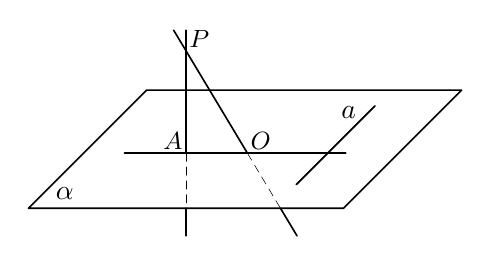
\begin{tikzpicture}[>=latex,scale=1.0,inner sep=1pt]
  \tkzDefPoints{0/0/A',4/0/B',5.5/1.5/C',1.5/1.5/D',2.0/2.0/P,2.0/0.7/A,3.2/0/D,2.0/0/E,1.8/0.7/F,3.4/0.3/M,4.4/1.3/N}
  \tkzDrawPolygon[semithick](A',B',C',D')
  \tkzInterLL(P,D)(A,F)\tkzGetPoint{O}
  \tkzDrawLines[add=0 and 0.2,semithick](A,P O,P)
  \tkzDrawLines[add=-1 and 0.5,semithick](A,E)
  \tkzDrawSegments[densely dashed](A,E O,D)
  \tkzDrawSegments[semithick](M,N)
  \tkzLabelLine[pos=0.8,above left](M,N){$a$}
  \tkzDrawLines[add=-1 and 0.5,semithick](O,D)
  \tkzDrawLines[semithick,add=1.0 and 1.6](A,O)
  \tkzLabelAngle[pos=0.5](B',A',D'){$\alpha$}
  \tkzLabelPoints[above right](P,O)
  \tkzLabelPoints[above left](A)
\end{tikzpicture}
\end{document}